\documentclass[12pt,letterpaper]{article}

% Paquetes esenciales   
\usepackage[utf8]{inputenc}
\usepackage[T1]{fontenc}
\usepackage[spanish]{babel}
\usepackage[top=1in, bottom=1in, left=1in, right=1in]{geometry}
\usepackage{graphicx}
\usepackage{hyperref}
\usepackage{enumitem}
\usepackage{tabularx}
\usepackage{booktabs}
\usepackage{xcolor}
\usepackage{colortbl}
\usepackage{fancyhdr}
\usepackage{titlesec}
\usepackage{lastpage}
\usepackage{listings}
\usepackage{listingsutf8}
\usepackage{courier} % Fuente monoespaciada

% Configuración para bloques de código
\lstdefinestyle{firewall}{
    backgroundcolor=\color{gray!5},
    commentstyle=\color{green!60!black}\bfseries,
    keywordstyle=\color{azuloscuro}\bfseries,
    numberstyle=\tiny\color{gray},
    stringstyle=\color{red!70!black},
    basicstyle=\ttfamily\small,
    breaklines=true,
    captionpos=b,
    keepspaces=true,
    numbers=left,
    numbersep=8pt,
    showspaces=false,
    showstringspaces=false,
    showtabs=false,
    tabsize=2,
    frame=single,
    rulecolor=\color{azulclaro},
    xleftmargin=15pt,
    xrightmargin=5pt,
    framexleftmargin=10pt,
    inputencoding=utf8
}

% Definición de colores
\definecolor{azuloscuro}{RGB}{0,51,102}
\definecolor{azulclaro}{RGB}{0,102,204}
\definecolor{grisoscuro}{RGB}{64,64,64}

% Configuración de hipervínculos
\hypersetup{
    colorlinks=true,
    linkcolor=azuloscuro,
    urlcolor=azulclaro,
    citecolor=azuloscuro
}

% Formato de títulos de sección con color
\titleformat{\section}
  {\color{azuloscuro}\Large\bfseries}
  {\thesection}{1em}{}

\titleformat{\subsection}
  {\color{azulclaro}\large\bfseries}
  {\thesubsection}{1em}{}

% Configuración de encabezado y pie de página
\setlength{\headheight}{24.01996pt}
\pagestyle{fancy}
\fancyhf{} % Limpiar encabezado y pie
\fancyhead[L]{\small\textcolor{grisoscuro}{Actividad 1 - Infraestructura de defensa}}
\fancyhead[R]{\small\textcolor{grisoscuro}{\nombreestudiante}}
\fancyfoot[C]{\small\textcolor{grisoscuro}{Página \thepage\ de \pageref{LastPage}}}
\renewcommand{\headrulewidth}{0.5pt}
\renewcommand{\footrulewidth}{0.5pt}
\renewcommand{\headrule}{\hbox to\headwidth{\color{azulclaro}\leaders\hrule height \headrulewidth\hfill}}
\renewcommand{\footrule}{\hbox to\headwidth{\color{azulclaro}\leaders\hrule height \footrulewidth\hfill}}

% Estilo para la primera página
\fancypagestyle{firstpage}{
  \fancyhf{}
  \fancyfoot[C]{\small\textcolor{grisoscuro}{Página \thepage\ de \pageref{LastPage}}}
  \renewcommand{\headrulewidth}{0pt}
  \renewcommand{\footrulewidth}{0.5pt}
  \renewcommand{\footrule}{\hbox to\headwidth{\color{azulclaro}\leaders\hrule height \footrulewidth\hfill}}
}

% Información del estudiante (modificar aquí)
\newcommand{\nombreestudiante}{Josué David Hernández Ramírez}
\newcommand{\fechaentrega}{Semana 6}

\begin{document}
\thispagestyle{firstpage}

% Portada con cuadro de información
\begin{center}
\colorbox{azuloscuro}{
\begin{minipage}{0.9\textwidth}
\vspace{0.3cm}
\centering
\textcolor{white}{\Large\textbf{ACTIVIDAD 1}}\\
\vspace{0.2cm}
\textcolor{white}{\large Infraestructura de defensa: Diseño de seguridad en redes}
\vspace{0.3cm}
\end{minipage}
}
\end{center}

\vspace{0.5cm}

% Datos del estudiante en cuadro
\noindent
\colorbox{gray!10}{
\begin{minipage}{\textwidth}
\textbf{\textcolor{azuloscuro}{Datos del estudiante}}

\textbf{Nombre y apellidos:} \nombreestudiante

\textbf{Fecha de entrega:} \fechaentrega
\end{minipage}
}

\section{\textcolor{azuloscuro}{Objetivos de la actividad}}
El presente documento detalla el diseño e implementación de una infraestructura de seguridad robusta para una organización que presta servicios a terceros, manejando información sensible y confidencial. La arquitectura propuesta integra múltiples capas de seguridad, incluyendo firewalls, sistemas IDS/IPS, VPN, y seguridad inalámbrica, garantizando la protección de datos y la continuidad operativa.

La organización cuenta con:

\begin{itemize}[leftmargin=*]
    \item Un centro de Procesamiento de Datos (CPD).
    \item Servdores web y de base de datos.
    \item Sistema de backup y mirror.
    \item Equipos portátiles para trabajo remoto.
\end{itemize}

\section{\textcolor{azuloscuro}{Diseño de Arquitectura de Seguridad}}

\begin{figure}[ht]
    \centering
    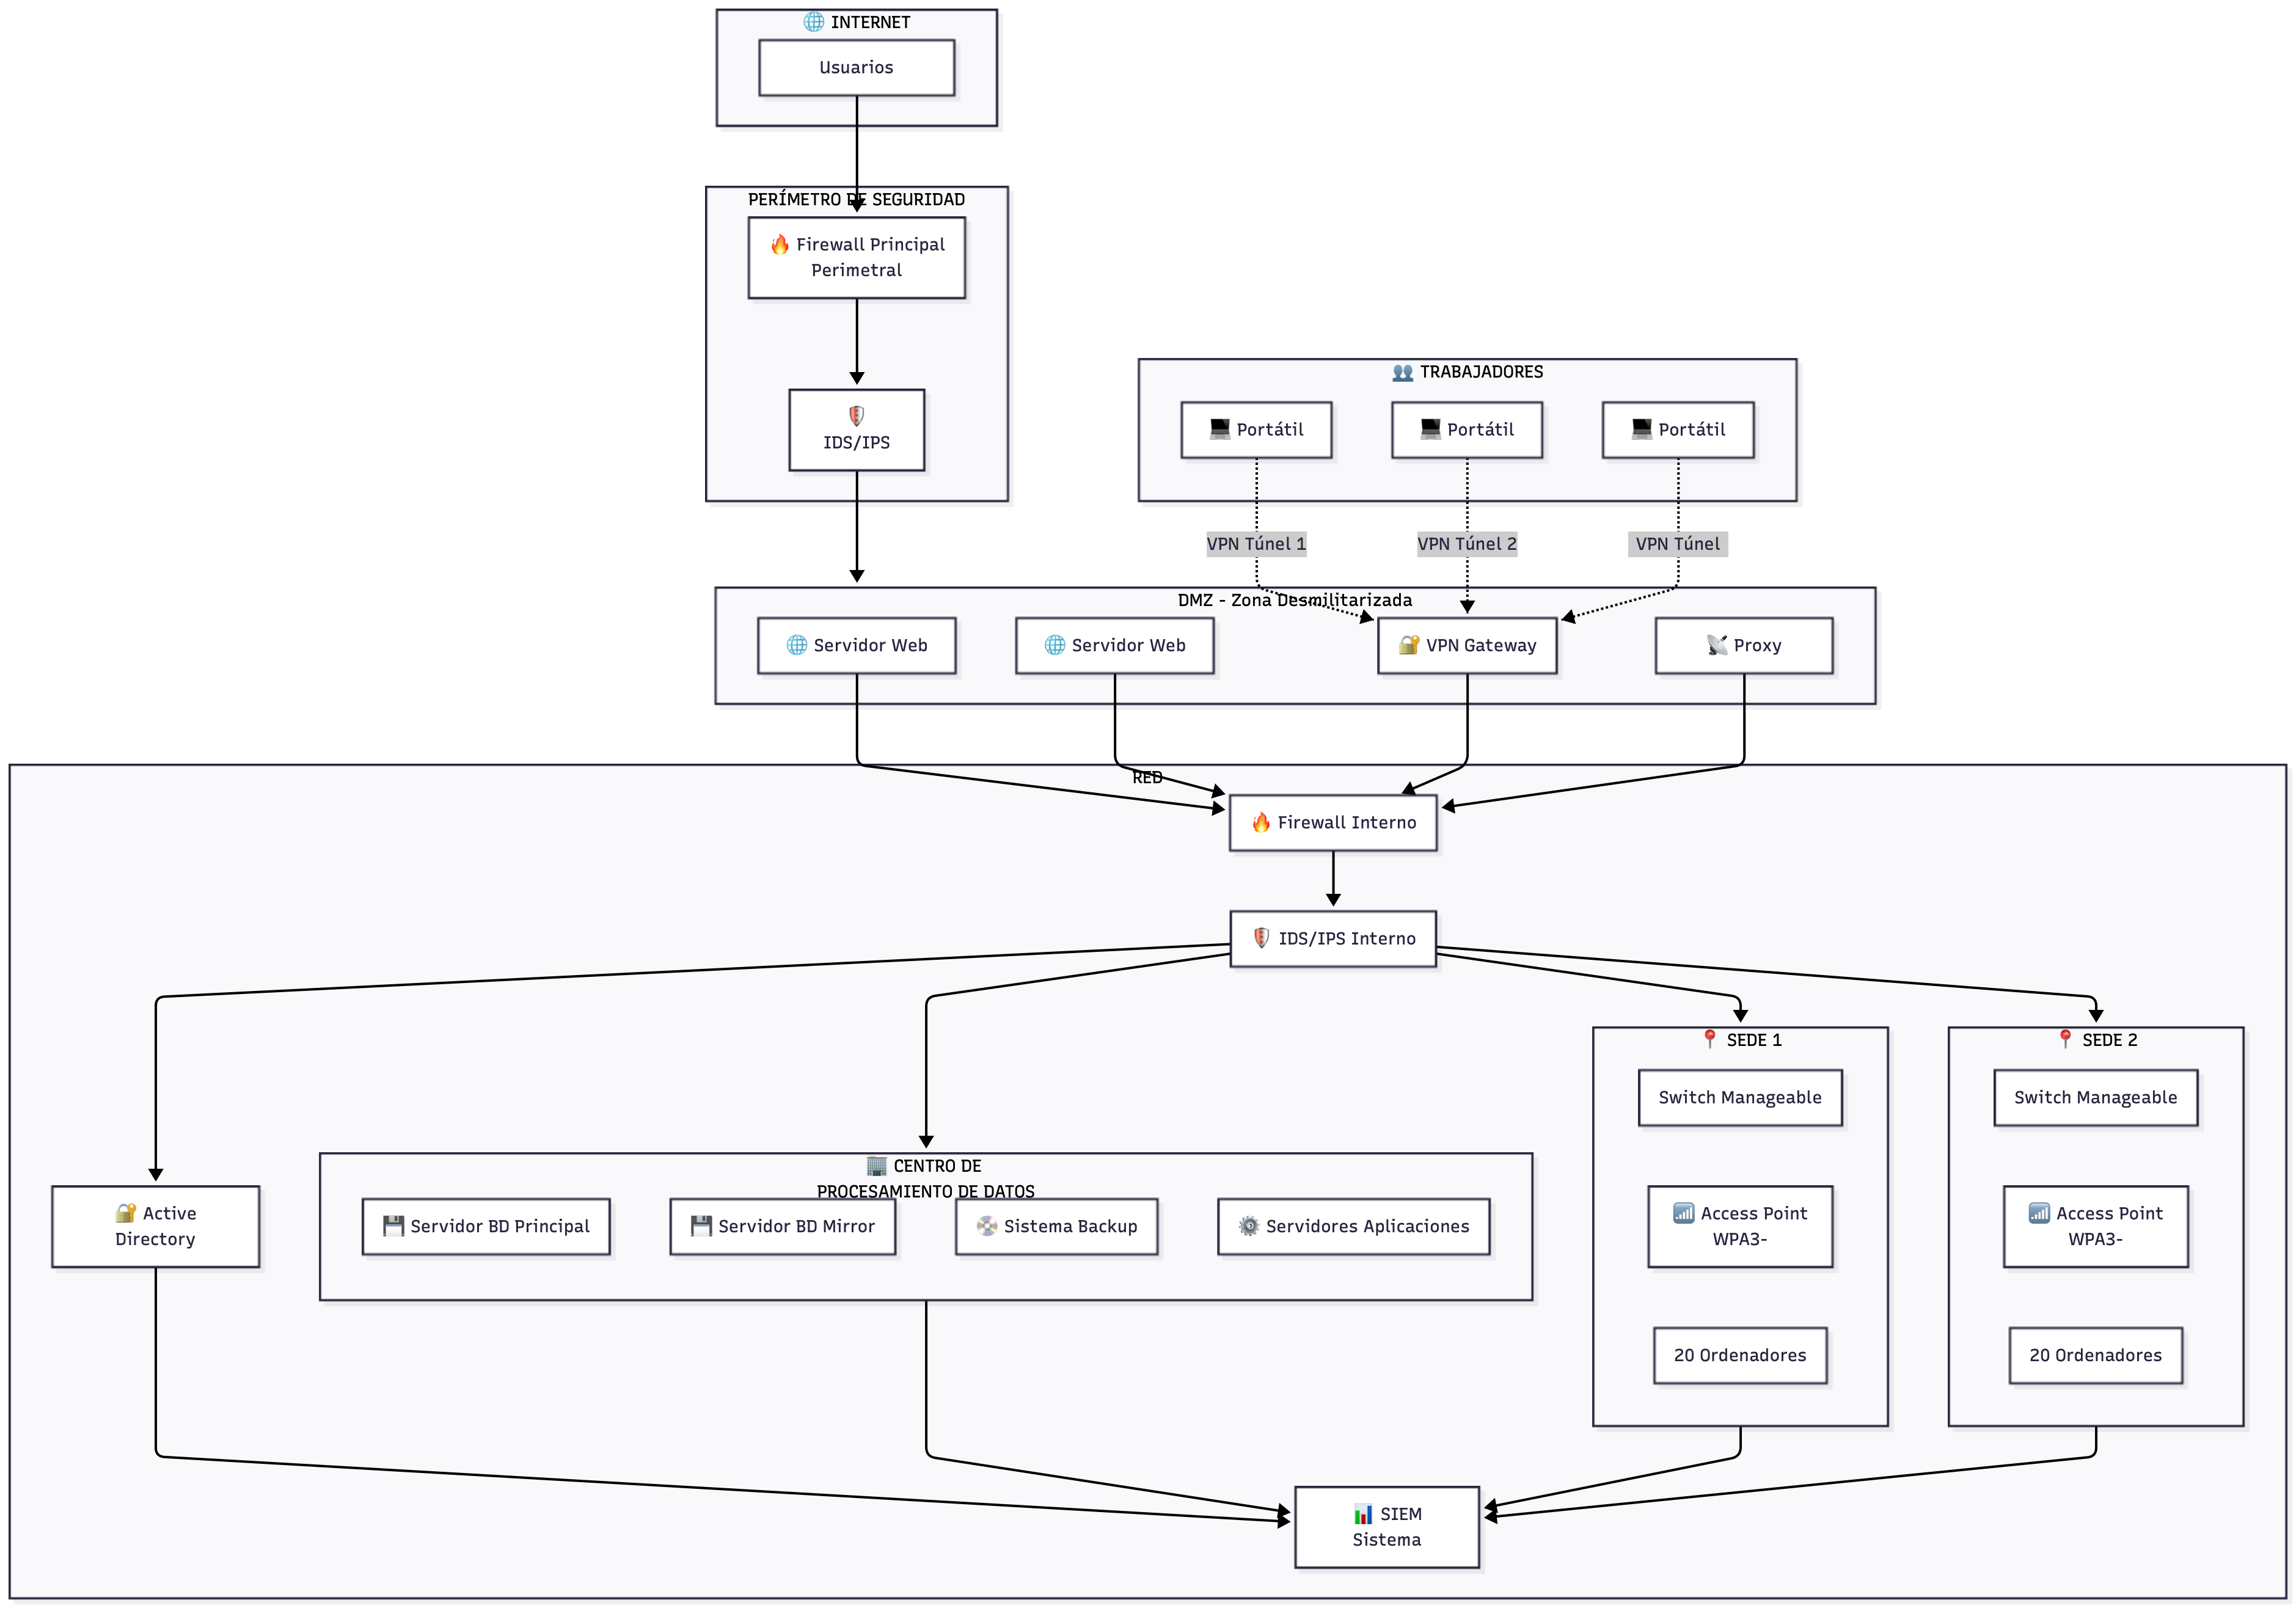
\includegraphics[width=0.9\textwidth]{./images/diagram.png}
    \caption{Diagrama de red}
    \label{fig:diagrama}
\end{figure}

\subsection{\textcolor{azuloscuro}{Segmentación de la Red}}

La arquitectura implementa una segmentación en capas que incluye:

\noindent\textbf{Capa 1 - Perímetro externo:}
\begin{itemize}
    \item Firewall perimetral (FW1) como primera línea de defensa.
    \item IDS/IPS en modo inline para análisis de tráfico entrante.
\end{itemize}

\noindent\textbf{Capa 2 - Zona Desmilitarizada:}
\begin{itemize}
    \item Servidores web con acceso público controlado.
    \item VPN Gateway para conexiones remotas.
    \item Proxy server para gestión de tráfico saliente.
\end{itemize}

\noindent\textbf{Capa 3 - Red Interna:}
\begin{itemize}
    \item Firewall interno (FW2) protegiendo recursos críticos.
    \item Segmentación por VLANs:
    \begin{itemize}
        \item VLAN 10: CPD y servidores críticos
        \item VLAN 20: Sede 1
        \item VLAN 30: Sede 2
        \item VLAN 40: Gestión y administración.
        \item VLAN 50: Wireless.
    \end{itemize}
\end{itemize}

\noindent\textbf{Capa 4 - CPD (Centro de Procesamiento de Datos):}
\begin{itemize}
    \item Máximo nivel de seguridad.
    \item Acceso controlado mediante ACLs estrictas.
    \item Sistemas de respaldo y redundancia.
\end{itemize}

\section{\textcolor{azuloscuro}{Configuración de Firewalls}}
\subsection{\textcolor{azuloscuro}{Firewall perimetral (FW1)}}

\noindent Tecnología: Firewall Next-Generation (NGFW) - Fortinet FortiGate o Palo Alto

\noindent\textbf{Reglas de Filtrado:}
\begin{lstlisting}[style=firewall, caption={Reglas del Firewall Perimetral}, escapeinside={(*@}{@*)}]
    # POL(*@\'{I}@*)TICA POR DEFECTO: DENEGAR TODO
    # Regla 1: Permitir HTTPS hacia servidores web DMZ
    Origen: ANY
    Destino: WEB1, WEB2 (DMZ)
    Puerto: 443/TCP
    Acci(*@\'{o}@*)n: PERMITIR
    Log: S(*@\'{I}@*)
    Inspecci(*@\'{o}@*)n: Deep Packet Inspection (DPI)
    
    # Regla 2: Permitir HTTP hacia servidores web DMZ (redirigir a HTTPS)
    Origen: ANY
    Destino: WEB1, WEB2 (DMZ)
    Puerto: 80/TCP
    Acci(*@\'{o}@*)n: PERMITIR (redirect to 443)
    Log: S(*@\'{I}@*)
    
    # Regla 3: Permitir VPN IPSec
    Origen: ANY
    Destino: VPN_GW
    Puerto: 500/UDP, 4500/UDP, ESP Protocol
    Acci(*@\'{o}@*)n: PERMITIR
    Log: S(*@\'{I}@*)
    Inspecci(*@\'{o}@*)n: Verificar certificados
    
    # Regla 4: Permitir DNS saliente (desde Proxy)
    Origen: PROXY (DMZ)
    Destino: ANY
    Puerto: 53/UDP, 53/TCP
    Acci(*@\'{o}@*)n: PERMITIR
    Log: S(*@\'{I}@*)
    
    # Regla 5: Bloquear pa(*@\'{i}@*)ses de alto riesgo
    Origen: Lista Geo-IP (Pa(*@\'{i}@*)ses bloqueados)
    Destino: ANY
    Acci(*@\'{o}@*)n: DENEGAR
    Log: S(*@\'{I}@*)
    Alerta: Enviar a SIEM
    
    # Regla 6: Rate Limiting para prevenir DDoS
    Origen: ANY
    Destino: DMZ
    L(*@\'{i}@*)mite: 1000 conexiones/minuto por IP
    Acci(*@\'{o}@*)n: DENEGAR exceso
    Log: S(*@\'{I}@*)
    
    # Regla 7: Denegar todo lo dem(*@\'{a}@*)s
    Origen: ANY
    Destino: ANY
    Acci(*@\'{o}@*)n: DENEGAR
    Log: S(*@\'{I}@*)
\end{lstlisting}

\noindent Características Avanzadas:
\begin{itemize}
    \item Protección anti-DDoS integrada.
    \item SSL/TLS Inspection para tráfico cifrado.
    \item Application Control (control de aplicaciones por firma).
    \item Web Filtering (categorización de URLs).
    \item Antivirus y Anti-malware en gateway.
\end{itemize}

\subsection{\textcolor{azuloscuro}{Firewall interno (FW2)}}
\noindent\textbf{Tecnología:} Firewall de próxima generación con capacidades de microsegmentación.

\noindent\textbf{Reglas de Filtrado:}
\begin{lstlisting}[style=firewall, caption={Reglas del Firewall Interna}, escapeinside={(*@}{@*)}]
    # POL(*@\'{I}@*)TICA POR DEFECTO: DENEGAR TODO

    # Regla 1: Permitir acceso DMZ a Servidores BD (solo consultas)
    Origen: WEB1, WEB2 (DMZ)
    Destino: DB_MAIN, DB_MIRROR (CPD)
    Puerto: 3306/TCP (MySQL), 5432/TCP (PostgreSQL)
    Acci(*@\'{o}@*)n: PERMITIR
    Log: S(*@\'{I}@*)
    Horario: 24/7
    Inspecci(*@\'{o}@*)n: Query validation

    # Regla 2: Permitir acceso Sedes a Servidores Aplicaciones
    Origen: VLAN 20 (Sede1), VLAN 30 (Sede2)
    Destino: APP (CPD)
    Puerto: 8080/TCP, 8443/TCP
    Acci(*@\'{o}@*)n: PERMITIR
    Log: S(*@\'{I}@*) 
    Autenticaci(*@\'{o}@*)n: Verificar con AD

    # Regla 3: Permitir VPN a recursos internos
    Origen: VPN_USERS (autenticados)
    Destino: VLAN 20, VLAN 30, APP
    Puerto: Seg(*@\'{u}@*)n perfil de usuario
    Acci(*@\'{o}@*)n: PERMITIR
    Log: S(*@\'{I}@*)
    2FA: REQUERIDO

    # Regla 4: Permitir gesti(*@\'{o}@*)n centralizada
    Origen: VLAN 40 (Gesti(*@\'{o}@*)n)
    Destino: ALL
    Puerto: 22/TCP (SSH), 3389/TCP (RDP), 443/TCP (HTTPS mgmt)
    Acci(*@\'{o}@*)n: PERMITIR
    Log: S(*@\'{I}@*)
    Origen espec(*@\'{i}@*)fico: Solo IPs de administradores

    # Regla 5: Denegar acceso directo a CPD desde Wireless
    Origen: VLAN 50 (Wireless)
    Destino: VLAN 10 (CPD)
    Acci(*@\'{o}@*)n: DENEGAR
    Log: S(*@\'{I}@*)
    Alerta: ALTA

    # Regla 6: Permitir backup schedule
    Origen: DB_MAIN, DB_MIRROR
    Destino: BACKUP
    Puerto: Protocolo backup (custom)
    Acci(*@\'{o}@*)n: PERMITIR
    Horario: 02:00-04:00 AM
    Log: S(*@\'{I}@*)

    # Regla 7: Permitir sincronizaci(*@\'{o}@*)n DB Mirror
    Origen: DB_MAIN
    Destino: DB_MIRROR
    Puerto: 3306/TCP, puerto replicaci(*@\'{o}@*)n
    Acci(*@\'{o}@*)n: PERMITIR
    Log: S(*@\'{I}@*)
    Cifrado: TLS obligatorio

    # Regla 8: Denegar todo lo dem(*@\'{a}@*)s
    Origen: ANY
    Destino: ANY
    Acci(*@\'{o}@*)n: DENEGAR
    Log: S(*@\'{I}@*)
\end{lstlisting}

\section{\textcolor{azuloscuro}{Implementación de IDS/IPS}}
\subsection{\textcolor{azuloscuro}{Sistema IDS/IPS de Entrada}}
\noindent Tecnología: Snort / Suricata en modo IPS inline
\noindent Ubicación: Entre Firewall perimetral y DMZ
\end{document}